\documentclass[Bachelorarbeit.tex]{subfiles}
%to translate single chapters
%	comment out first line
%	insert following two lines
%\documentclass[a4paper,12pt]{report}
%\usepackage{../sty/fhv}

\begin{document}
\chapter{Problem description}\label{ProblemDescription}
\section{Overview}
According to the articel  \textit{Face recognition: A literature survey} from \cite{FRLiteratureSurvey}, face recognition can be segmented into three key steps, shown in figure \ref{FRP}.\\

\begin{figure}[!h]
\centering
\includegraphics[page=2,width=14cm]{./pictures/drawings_2}
\caption{Face Recognition Progress \label{FRP}}
\end{figure}

\textbf{Face Detection} is responsible for a rough normalization (like face tracking) and use for this task different approaches.\\
\textbf{Face Extraction} generates a more accurate normalization (like human emotions). The different approaches to get this emotions are shown in figure \ref{FRP}. Face detection and face extraction approaches can use the same feature-based-method (like informations out of color, Motion, ...)so they can perform simultaneous. \\
\textbf{Face Recognition} is the last step to identify/verify a picture. For a verification/identification several methods are available.


\section{Face Detection}
We decided to have a closer look on the face detection process because for the processes afterwards we need a detected face, which is not available without any effort.
\\To find an approach which we can study, implement and test we made further researches in this segment. The article \textit{Face detection: A survey} from \cite{FDASurvey} gives a good overview of the topic face detection. The figure \ref{FDaS} (out of \cite{FDASurvey}) represents the different approaches to detect faces in a picture.\\

\begin{figure}[!h] %Face Detection detaild approaches
\centering
\includegraphics[page=3, width=14cm]{./pictures/drawings_2}
\caption{Face Detection divided into approaches (more detailed from \cite{FDASurvey}). \label{FDaS}}
\end{figure}

According to \cite{FDASurvey} are \textbf{Image-based approaches} the moste robust techniques for gray images, but on the other side they need a lot of computation time by multiresolution window scanning.\\
The \textbf{feature-based approaches} were the first attemps in the face detection history. They are built up simple and so they need less computation time, this enables these approaches access to real-time applications.

The most interesting approach for us was \textit{Face detection based on color likelihood} approach (in figure \ref{FDaS} marked as \textit{Color}). Argumentation for this algorithm can be found in the section \ref{cbFd};


\section{Color based face detection} \label{cbFd}
According to the article \textit{A Robust Skin Color Based Face Detection Algorithm} of \cite{RobustSkinColorFD} following points argue for the color based case detection
\begin{itemize}
\item Color processing is much faster than other facial features
\item Color based algorithm is orientation invariant, that means that a motion estimation is much easier.
\item Color based algorithm is often the first step for detection, this algorithm is popular.
\end{itemize}

An application for the simple and real-time capable algorithmus face detection with color can be found in the articel  \textit{Face recognition: A literature survey} from \cite{FRLiteratureSurvey}
\begin{quotation}
\textit{In video conferencing systems, there is a need to automatically control the camera in
such a way that the current speaker always has the focus. One simple approach to this
is to guide the camera based on sound or simple cues such as motion and skin color.}
\end{quotation}
\end{document}
